%-------------------------------------------------------
% Methodology
%-------------------------------------------------------
\section{Methodology}
\label{sec:methodology}

%----------------------------------------------
% * Verwendetet Technologien
%----------------------------------------------
\subsection{Verwendetet Technologien und Protokolle}
\label{sec:Verwendetet Technologien}
Bevor auf die eigentliche Umsetzung eingegangen wird werden noch kurz die verwendeten Frameworks und Technologien erklärt.
Ein Teil davon wie HTTP und Rest wurden bereits durch das Interface für KRESHMOI festgelegt, ein weiter ergab sich durch die Anforderung einer Web-Applikation.
Die Frameworks und Technologien für Grafik und GUI wurden gewählt weil mit Ihnen eine schnelle Umsetzung der Anforderungen möglich war.

%----------------------------------------------
% ** HTTP
%----------------------------------------------
\subsubsection{HTTP}
\label{sec:HTTP}
HTTP (Hyper Text Transfer Protokoll) ist ein Protokoll zur übertragung von Daten über ein Netzwerk welches auf TCP aufsetzt.
Der Datenaustausch zwischen zwei Kommunikationspartner findet in der From von Nachrichten statt, 
wobei der Client eine Anfrage an einen Server stellt und dieser die Anfrage bearbeitet und eine Antwort retuniert.
%
Eine Nachricht setzt sich aus einem Header und einen Body zusammen.
Der Body enthält die Nutzdaten und der Header enthält Metadaten über die Nutzdaten.
Vom Aufbau der Nachricht unterscheiden sich Anfrage und Antwort nur in der ersten Zeile:
\begin{itemize}
	\item Anfrage: Enthält die HTTP-Methode, die URL welche auf die Resource am Server zeigt und die Protokollversion.
	\item Antwort: Enthält die Protokollversion und den Serverstatus. 
		Der Serverstatus liefert eine Aussage ob der Request erfolgreich bearbeitet wurde bzw welche Art von Fehler bei der Bearbeitung aufgetreten ist.
\end{itemize}
HTTP ist ein zustandsloses Protokoll, daher wird nach jeder Anfrage die Verbindung vom Server wieder abgebaut.
Für eine Zuordnung eines Clients muss dieser eine Session-ID mitsenden welche normalerweise im Header enthalten ist \cite{http}.

%--------------------------------------------- 
% ** REST
%----------------------------------------------
\subsubsection{REST}
\label{sec:HTTP}
REST ist im eigentlichen Sin mehr ein Architekturstiel als ein Protokoll welcher mit HTTP umgesetzt wird.
Die Idee von REST ist dass eine URL genau eine Resource auf einem Server addressiert, 
wobei eine Resource eine statische Datei oder das ergebniss einer aktion auf dem Server sein kann.
Der Architekturstiel ist lässt sich durch fünf Prizipien zusammenfassen:
\begin{itemize}
	\item \textbf{Resource mit eindeutiger Identifikation:}
		Jede Resrouce wird durch eine URI (Uniform Resouce Identifier) weltweit eindeutig identifiziert.
		Diese addressiert unter anderem den Server auf den sich die resource befindet sowie Resource auf dem Server selbst.
	\item \textbf{Hypermedia:}
		Verknüfungen zu anderen Entitäten und werden als Links auf die jeweiligen Resourcen dargestellt.
		Weiters kann die Steuertung des Applikationszustandes durch Links auf weiter Aktionen durch Hypermedia umgesetzt werden.
	\item \textbf{Standard-Opperationen:}
		Es gibt ein definiertes Interface welches von jeder Resource zur verfügung gestellt werden muss.
		Dieses umfasst einen relativ kleinen Satz von Opperationen welche auf die Resource ausgeführt werden können.
	\item \textbf{Unterschiedliche repräsentation der Resourcen:}
		Die Resourcen können unterschiedliche Darstellungsformen haben.
		Ein Client kann also eine Resource in einem bestimmten Format (z.B.: XML, HTML, JSON) anfordern sofern diese Darstellung vom Server unterstüzt wird.
		In HTTP wird die gewünschte Dartstellung im Header angegeben.
	\item \textbf{Zustandslose Kommunikation}
		Der Server hällt keine Zustandsinformationen über den Client welcher über die Dauer eines Requests hinaus geht.
		Daher muss der Zustand einer Anwendung entweder am Client liegen oder vom Server in eine Resource umgewandelt werden.
\end{itemize}
\cite{rest}

%----------------------------------------------
% ** JSON
%----------------------------------------------
\subsubsection{JSON}
\label{sec:JSON}
Bei JSON (JavaScript Object Notation) handelt es sich um ein Datenformat zum Autausch von Arrays und Objekt-Graphen.
JSON findet neben XML vorallem in der Kommunikation zwischen Client und Server bei Webanwendungen Verwendung, 
wobei JSON Daten wesentlich kompakter und damit Resourcensparender sind.
Wie bei XML werden Listen und Objekte in einer von Menschen lesbaren Form darestellt.
Dabei werden folgende Datentypen unterstützt welche wiederum beliebig tief ineinander Verschachtelt werden können: NULL, Boolean, Zahl, String, Array und Objekt \cite{ajax}.

%----------------------------------------------
% ** AJAX
%----------------------------------------------
\subsubsection{AJAX}
\label{sec:AJAX}
AJAX (Asynchronous JavaScript and XML) ermöglicht es einer Webanwendung kleinere Mengen von Daten nachzuladen und damit Teile der Webseite dynamisch zu ändern, 
statt bei jeder Aktion die Webseite neu zu laden.
Benötigt die Web Appliketion Daten vom Server wird an diesem eine HTTP Anfrage gesendet und Callback-Funktionen für den Fall einer Antwort oder eines Fehlers beim Browser registriert.
Erhällt der Browser eine Antwort auf sine Anfrage ruft er die Callback-Funktion auf und übergibt die erhalten Daten wodurch die Webanwendung mit der Verarbeitung dieser fortfahren kann.
Dies ermöglicht die Entwicklung komplexer Webapplikationen, wobei die Webapplikation selbst mit der Seite geladen wird und die Daten die der Benutzer mit der Anwendung verarbeiten möchte dynamisch von dieser nachgeladen werden können \cite{ajax}.

%----------------------------------------------
% ** Objectiv J
%----------------------------------------------
\subsubsection{Objectiv J}
\label{sec:Objectiv J}

Objective J ist eine Programmiersprache welche sich von der Syntax stark an Objective C anlehnt.
Sie ist eine Erweiterung oder Obermenge von Javascript und wird von einem in Javascript geschriebenen Interpreter abgearbeitet.
In Javascript können Objekte durch Prototyping erstellt werden, das Konzept von Klassen wird aber nicht unterstüzt.
Obj J bietet zusätzlich zu den nativen JS Objekten die definition von Klassen inklusive Vererbung und die generierung von Objekten daraus.
Obwohl es die Sprache erlaubt für Variablen, Methodenparameter und Rückgaben eine Datentyp zu definieren, 
werden diese aufgrund von schwacher Typisierung vom Interpreter nicht auf ihre Einhaltung überprüft.
In der aktullen Version wird die Übergabe von Referenzen als Parameter ähnlich einem Pointer in C unterstützt \cite{capp}.

%----------------------------------------------
% ** Cappuccino
%----------------------------------------------
\subsubsection{Cappuccino}
\label{sec:Cappuccino}
Bei Cappuccino handelt es sich um ein Web Application Framework für Objectiv J und Javascript, welches haupsächlich der Erstellung komplexer Benutzeroberflächen dient.
Das Framework lehnt sich sowol vom Aussehen als auch von der Benennung der Komponenten sehr stark an das GUI-Framework Cocoa von Apple an.
GUI-Elemente werden als Objekte erstellt welche von einer View-Klasse erben und innerhalb von anderen Views positioniert werden können.
Das Interface wird von einem HTML5 fähigen Browser gerendert wobei für dessen Erstellung keinerlei HTML oder CSS kentnisse notwendig sind \cite{capp}.


%----------------------------------------------
% ** WebGL 
%----------------------------------------------
\subsubsection{WebGL}
\label{sec:WebGL}
WebGL ist eine API für die Erstellung von 2D und 3D Grafiken in Browsern mit der Unterstützung der Grafikkarte.
Im gegensatz zur Canvas-2D API wo die Bilder in der CPU gerendert werden, ist WebGL aufgrund der Hardwarebeschleunigung wesentlich performanter.
WebGL ist eine Shaderbasierte API welche sich sehr stark an OpenGL ES anlehnt.
Diese bedeutet dass Code für die Recheneinheiten (Shadereinheiten) der Grafikkarte entwickelt wird,
welchen der Treiber der Karte in Bytecode übersetzt und zur ausführung in den Grafikchip lädt.
Die Shaderprogramme werden in der Programmiersprache GLSL geschrieben welche sich sehr stark an C orientiert.
Der Zugriff auf die Schnittstelle erfolgt über das HTML Canvas Element in welchem die Ausgabe der Grafikkarte dargestellt wird.
Dies geschieht mittels JavaScript wo die API funktionen zur Übergabe der Nutzdaten, Befehle und der Shaderprogramme bereitstellt \cite{webgl-14}.

%----------------------------------------------
% ** PixiJS 
%----------------------------------------------
\subsubsection{PixiJS}
\label{sec:PixiJS}
Da WebGL eine relativ Hardware nahe API ist wurden einige Frameworks entwickelt welche von der Komplexität einer solchen API abstrahieren, zu denen auch PixiJS zählt.
Dies bietet Funktionen zum Zeichen von Geometrischen Figuren, Füllen von diesen und Laden von Texturen.
Eine Szene in PixiJS ist als Baum organisiert wobei jeder Knoten in dem Baum wiederum Operationen zur Manipulation wie Transformation, Translation oder Transparenz anbietet.
Ein weiteres Feature ist dass auf einen Knoten ein Filter mit WebGL Fragment-Shader-Code gesetzt werden kann welcher zur Manipulation der Farbinformation in den einzelnen Bildpunkte dient \cite{pixijs}.


%----------------------------------------------
% * Funktionalität und Aufbau der Benutzeroberfläche
%----------------------------------------------
\subsection{Funktionalität und Aufbau der Benutzeroberfläche}
\label{sec:Funktionalität und Aufbau der Benutzeroberfläche}
Der Workflow beim Durchsuchen von radiologischen Aufnahmen mit KRESHMOI gliedert sich in folgende Schritte:
\begin{enumerate}
	\item Auswahl eines Start-Datensatzes.
	\item Betrachen des Datensatzes.
	\item Anotieren einer ROI und eventuelle Eingagbe von Text in die Suchzeile.
	\item Suche absenden und Ergebniss listen.
	\item Betrachen von Datensätzen aus der Ergebnissliste.
	\item Um neue Suchanfrage von ein Ergebnissdatensatz aus zu stellen werden die Schritte von 3 an wiederholt.
\end{enumerate}
Entsprechend dieses Ablaufs wird beim start der Applikation eine Liste mit allen Datensätzen geladen, 
aus welchen einer als Einstiegspunkt in die Suche ausgewählt werden kann.
Dieser Datensatz wird in den Betrachter der Haupansicht geladen.
Die Haupansicht setzt sich aus verschiedenen Interaktions-Elementen (Views) zusammen,
welchen in mehreren möglichen Layouts mit unterschiedlicher Multiplizität und Anordnung miteinander kombiniert werden.
Von diesen Elementen gibt es Vier verschiedene Typen:
\begin{itemize}
	\item Betrachtungsansicht für Volumes (2D-Betrachter)
	\item Betrachtungsansicht für den Report (Report-Betrachter)
	\item Präsentationsansicht für die Ergebnisse (Ergebniss-Liste)
	\item Eingabezeile für Schagwörter mit dem Suchbutton (SuchzeilSuchzeilee)
\end{itemize}
Die Fläche welchen die einzelnen Views innerhalb des Browserfensters einnehmen kann zwischen ihnen beliebig verschoben werden, 
unter der Prämisse dass die Bedienelemente der einezlenen Views genügend Platz haben.
Auf den Funktionsumfang des 2D-Betrachters und der Ergebniss-Liste wird in den folgenden unterkapiteln etwas genauer eingegangen.
\begin{figure}[t]
	\centering
		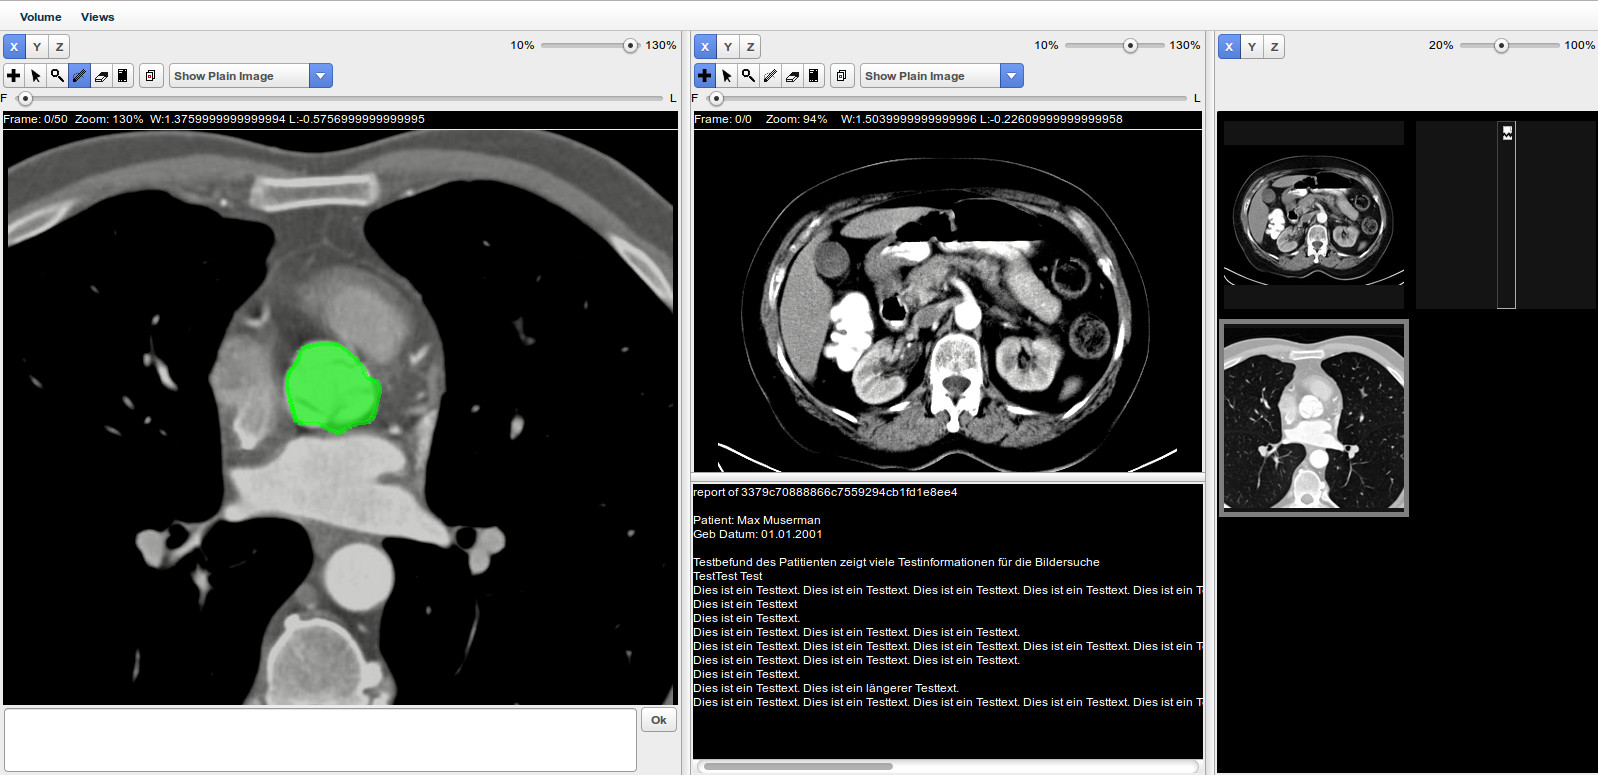
\includegraphics[width=0.8\linewidth]{img/c3_application_standard.jpg}
	\caption{Hauptansicht mit Layout für zwei 2D-Betrachter, Report-Betrachter und Ergebniss-Liste}
\end{figure}


%----------------------------------------------
% ** Funktionalität des 2D-Betrachters
%----------------------------------------------
\subsubsection{Funktionalität des 2D-Betrachters}
\label{sec:Funktionalität des 2D-Betrachters}
Der 2D-Betrachter orientiert sich von seinen Funktionen sehr stark an der Betrachtungssoftware einer PACS-Workstaion oder eines DICOM-Betrachters.
Er ermöglicht die räumliche Naviation durch die Schnitte eines Volumes in einer bestimmten Orientierung sowie das Umschalten zwischen den Orientierungen.
Weiter kann wenn das Volume aus der Ergebnissliste ausgewählt wurde, 
also nicht der Startdatensatz ist,
eine Anzeige mit den Deckungsbereichen der Suche hinzugeschaltet werden. 

Zur Interaktion mit den Volume wird auch wie bei anderen Betrachtern der Maus eine bestimmte Funktion zugewiesen.
Die Funktionen umfassen Fensterung, Zoom, Bewegen des Bildes und Zeichnen und Löschen von Polygonen (ROIs).
Das Einzeichenen von ROIs ist um die Benutzung einfach zu halten auf ein einelnes Schnittbild beschränkt.
Wird das Werkzeug zum Zeichen oder Löschen von Polygonen auf mehreren Schnitten verwendet springt der Betrachte bei deren Verwendung immer wieder auf das Schnittbild mit dem ersten Polygon zurück.
Das Bild kann Halbtransparent mit dem Report des Datensatzes überblendet werden, was aber die Mausfunktion auf das Scrollen des Reports reduziert.
In allen anderen Funktionen ist das Scrollen immer an die Navigation durch die Schnitte gebunden.

%----------------------------------------------
% ** Funktionalität der Ergebniss-Liste
%----------------------------------------------
\subsubsection{Funktionalität der Ergebniss-Liste}
\label{sec:Funktionalität der Ergebniss-Liste}
Die Ergebniss-Liste präsentiert die Ergebnisse einer Suche welches sie über Drag and Drop in einen Betrachter laden lassen.
Die Präsentation erfolgt über ein Vorschaubild welches von KRESHMOI als repräsentaties Bild für die Suche gewählt wurde.
Um ein Suchergebniss im vorfeld zu Beurteilen verfügt die Ergebniss-List ebenfalls über die funktion die Orientierung der Schnitte des Volumes zu ändern und die Vorschaubilder zu zoomen.



%----------------------------------------------
% * Kommunikation mit KRESHMOI
%----------------------------------------------
\subsection{Kommunikation mit KRESHMOI}
\label{sec:Kommunikation mit KRESHMOI}
Der Datenaustausch mit KRESHMOI basiert auf REST wobei sowohl auf die einzelnen Slices von einem Volume, als auch auf die Suche als Resoure über eine URL zugegrifen werden kann.

%----------------------------------------------
% ** Query nach Bildern
%----------------------------------------------
\subsubsection{Query nach Bildern}
\label{sec:Query nach Bildern}
Der Zugriff auf die Suchfunktion erfolgt über eine POST-Operation in welcher die Anfrage und die Antwort in JSON codiert werden.
Zum Ausführen einer Suchanfrage stehen zwei Resourcen zur verfügung:
\\
\\
\textit{/index}\\
Liefert ein Array von allen Verfügbaren Datensätzen zurück 
\\
\\
\textit{/query}\\
Liefert ein Array von Datensätzen zurück welche anhand der Übergebenen Suchkriterien gefunden wurden.
Eine Suchanfrage basiert immer auf einen Datensatz welcher in der Anfrage übergeben werden muss.
In diesem Datensatz werden weiters Interessante Bereiche sogenannte ROIs (Region of Interesst) in den einzelnen Schnittbildern definiert.
Die Übergabe einer ROI erfolgt als Polygon in Form einer Listen von Punkten im drei Dimensionalen Raum des Volumes.
\begin{lstlisting}[
	language=json,
	firstnumber=1,
	caption=Query
]
{
   "queryid":"",
   "text":"",
   "imageid":"",
   "roi": 
   [
      "polygon":
      [
         "point":{"x":0, "y":1, "z":0},
         "point":{"x":1, "y":1, "z":0},
         "point":{"x":0, "y":0, "z":0}
      ],

   ]
}
\end{lstlisting}


\begin{lstlisting}[
	language=json,
	firstnumber=1,
	caption=Result
]
{
   "rankedImageID": 
   [
      {
         "imageID": "9587336b132b127b936ad0afd80ca862",
         "normalDimX": 52,
         "normalDimY": 512,
         "normalDimZ": 512,
         "relevance": 1,
         "report": "",
         "title": "Some Image"
      },
   ]
}
\end{lstlisting}

%----------------------------------------------
% ** Laden der Bilder
%----------------------------------------------
\subsubsection{Laden der Bilder}
\label{sec:Laden der Bilder}
Die Bildaten eines Volumes können über eine GET-Operation geladen werden.
Dabei wird jedes Volume als eine Resource im Unterverzeichniss \textit{/image/} indentifiziert.
Über Parameter in der URL werden die Schnittrichtung und und die Nummer des Bildes in der jeweiligen Schnittebene angegeben.
Wir keine Nummer für das Bild angegeben wählt KRESHMOI eine repräsentatives Bild für die Suchanfrage, welches für die Präsentation der Ergebnisse verwendet wird.
Für die Schnittebene gibt es entrsprechende der Terminologie für die Bildgebung in der Anatomie die Optionen:
\begin{itemize}
	\item Axial: Die Schnitte erfolgen Wagrecht in der Transversalebene
	\item Sagital: Die Schnitte erfolgen Senkrecht in der Sagitalebene
	\item Coronal: Die Schnitte erfolgen Senkrecht in der Frontalebene 
\end{itemize}
Sollen die Regionen welche der Suchanfrage entsprechen in den einzelnen Bildern markiert werden, muss die Query-ID mit übergeben werden um die urspüngliche Suchanfrage zu identifizieren.
\\
\\
Beispiel:
\\
\url{/image/9587336b132b127b936ad0afd80ca86.jpg?slice=1&direction=axial&query=1}
%TODO: Prüfen ob URL ok
%TODO: Zitieren von KRESHMOI API
%TODO: Zitieren der Schnittebenen
%TODO: Bild ist wikipedia ok: http://de.wikipedia.org/wiki/Anatomische_Lage-_und_Richtungsbezeichnungen

%----------------------------------------------
% * Architektur und Komponenten
%----------------------------------------------
\subsection{Architektur und Komponenten}
\label{sec:Architektur und Komponenten}

%----------------------------------------------
% ** Domänen Model
%----------------------------------------------
\subsubsection{Domänen Model}
\label{sec:Domänen Model}

%----------------------------------------------
% ** Architektur und Aufteilung in Komponenten
%----------------------------------------------
\subsubsection{Architektur und Aufteilung in Komponenten}
\label{sec:Architektur und Aufteilung in Komponenten}

%----------------------------------------------
% ** 2DView
%----------------------------------------------
\subsubsection{2DView}
\label{sec:2DView}


%----------------------------------------------
% ** Kommunikations Module
%----------------------------------------------
\subsubsection{Kommunikations Module}
\label{sec:Kommunikations Module}

%----------------------------------------------
% * Usability
%----------------------------------------------
\subsection{Usability}
\label{sec:Usability}

%----------------------------------------------
% ** Workflow bei der Befundung
%----------------------------------------------
\subsubsection{Workflow bei der Befundung}
\label{sec:Workflow bei der Befundung}

